% !TEX TS-program = pdflatex
% !TEX encoding = UTF-8 Unicode

% This is a simple template for a LaTeX document using the "article" class.
% See "book", "report", "letter" for other types of document.

\documentclass[11pt]{article} % use larger type; default would be 10pt

\usepackage[utf8]{inputenc} % set input encoding (not needed with XeLaTeX)

%%% Examples of Article customizations
% These packages are optional, depending whether you want the features they provide.
% See the LaTeX Companion or other references for full information.

%%% PAGE DIMENSIONS
\usepackage{geometry} % to change the page dimensions
\geometry{a4paper} % or letterpaper (US) or a5paper or....
% \geometry{margin=2in} % for example, change the margins to 2 inches all round
% \geometry{landscape} % set up the page for landscape
%   read geometry.pdf for detailed page layout information

\usepackage{graphicx} % support the \includegraphics command and options
\usepackage{subfig}
\usepackage[parfill]{parskip} % Activate to begin paragraphs with an empty line rather than an indent

%%% PACKAGES
\usepackage{booktabs} % for much better looking tables
\usepackage{array} % for better arrays (eg matrices) in maths
\usepackage{paralist} % very flexible & customisable lists (eg. enumerate/itemize, etc.)
\usepackage{verbatim} % adds environment for commenting out blocks of text & for better verbatim
\usepackage{subfig} % make it possible to include more than one captioned figure/table in a single float
% These packages are all incorporated in the memoir class to one degree or another...

%%% HEADERS & FOOTERS
\usepackage{fancyhdr} % This should be set AFTER setting up the page geometry
\pagestyle{fancy} % options: empty , plain , fancy
\renewcommand{\headrulewidth}{0pt} % customise the layout...
\lhead{}\chead{}\rhead{}
\lfoot{}\cfoot{\thepage}\rfoot{}

%%% SECTION TITLE APPEARANCE
\usepackage{sectsty}
\allsectionsfont{\sffamily\mdseries\upshape} % (See the fntguide.pdf for font help)
% (This matches ConTeXt defaults)

%%% ToC (table of contents) APPEARANCE
\usepackage[nottoc,notlof,notlot]{tocbibind} % Put the bibliography in the ToC
\usepackage[titles,subfigure]{tocloft} % Alter the style of the Table of Contents
\renewcommand{\cftsecfont}{\rmfamily\mdseries\upshape}
\renewcommand{\cftsecpagefont}{\rmfamily\mdseries\upshape} % No bold!

%%% END Article customizations

%%% The "real" document content comes below...

\title{Advanced Vision Assignment 2}
\author{Behzad Tabibian and Gintautas Sasnauskas}
\date{} % Activate to display a given date or no date (if empty),
         % otherwise the current date is printed 

\begin{document}
\maketitle

\section{Introduction}

For the second assignment of Advanced Vision course we implemented a system, which classifies motion images into three categories. Motion images in the dataset represent a hand showing one of three signs in rock-paper-scissors game. 

Solution for this problem was implemented in Python language using OpenCV library for processing images and MLPy library for classification.

\section{Implementation}

\subsection{Hand recognition}

When presented a motion sequence, moving hand is first detected in each image of the sequence. This is done in a number of steps.

At first image background is subtracted from the image. This allows us to only see things which have changed comparing to the background. Example of image from which background was subtracted is shown in Figure \ref{fig:bgsub},

Obtained image is then smoothened using median blur in order to reduce noise. Such image is then transformed into black and white image according to threshold based on a colour of a typical hand in the data set. Such colour is found to lie between RGB values of $(0, 0, 27)$ and $(100, 100, 140)$.

To improve precision of the background subtraction and to account for possible lighting changes between different sets of images, first image of the sequence is also subtracted from the image. This removes all static features from the image. Such static features are often artifacts caused by changed lighting conditions. Both, first image which is subtracted from image of interest and image of interest itself, are preprocessed in the same way.

\begin{math}
Image^*_n = f(Image_n - Background) - f(Image_1 - Background), n \geq 2
\end{math}



\subsection{Feature extraction}

Two sets of features are extracted from the motion picture image to be used in the classifier:

\begin{enumerate}
\item Hu Moments;
\item Changes in the area of the extracted object over time.
\end{enumerate}

\subsubsection*{Hu Moments}

Hu set of invariant moment is used as the first set of features. In order to calculate Hu moments, motion history image for a given video clip is first built. Motion history image is built from black and white images reconstructed from contour images by combining them into one image by superimposing them. Motion history images for "rock", "paper" and "scissors" signs are shown in Figure \ref{fig:mhir}, Figure \ref{fig:mhip} and \ref{fig:mhis} respectively. 

\begin{figure}
\begin{center}

\includegraphics[width=80mm]{mhi_rock.png}
\caption{Motion history image for "rock" sign.}
\label{fig:mhir}
\end{center}
\end{figure}

\begin{figure}
\begin{center}

\includegraphics[width=80mm]{mhi_paper.png}
\caption{Motion history image for "paper" sign.}
\label{fig:mhip}
\end{center}
\end{figure}

\begin{figure}
\begin{center}

\includegraphics[width=80mm]{mhi_scissors.png}
\caption{Motion history image for "scissors" sign.}
\label{fig:mhis}
\end{center}
\end{figure}

\subsubsection*{Temporal function of the object size}

In addition to Hu Moments, additional set of five features is generated by temporarily dividing provided video clip into five equal segments and calculating average area taken by the object in each of these segments. This way we can see how area of the hand in the image changes over time and represent such changes as features usable by the classifier. 

While being a simple method, it explains large amount of variance between different signs. 

\subsection{Classifier}

To classify different types of image sequence we used MLpy library. MLpy is Machine Learning library for python which provides a variety of ML algorithms and tools to perform ML on data.\\
The algorithm used in this project is Linear Support Vector Machine which trained over 5 principle components of the input data produced by previous section.
\subsubsection*{Principle Component Analysis}
Input vector consists of 12 features for every image sequence, 7 HuMoments and 5 Area measures over time. Dataset lies in 12 dimension space. We performed PCA on the input dataset to reduce dimensionality of the original dataset. Prior to Principal Component Analysis we normalize all the features to zero mean and standard deviation. In figure \ref{fig:pcaplot} we can see that only first 5 Principle Components contribute to most variation in the dataset and therefore input data sits on a lower dimension. \\Using these components we project the all the dataset and any other input data into lower 5 dimension subspace.\\

\begin{figure}[htp]
\begin{center}
\leavevmode
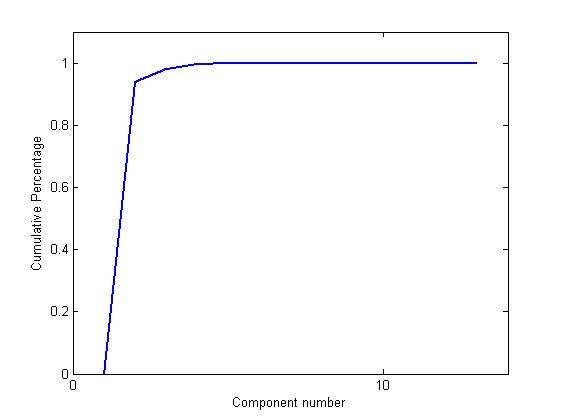
\includegraphics[width=0.6\textwidth] {pca.jpg}
\end{center}
\caption{Cumulative Percentage PCs}
\label{fig:pcaplot}
\end{figure}

\subsubsection*{SVM}
Projected data is then used to train a linear SVM. The algorithm is an implementation of multi-class support vector classification by Crammer and Singer. This algorithm is also available in MLpy library.\\
We also tested Logistic Regression, however as later results will show SVM outperformed. The results for both classifiers are presented in results section.
\subsubsection*{Cross Validation}
In order to evaluate performance of the classifier we utilized Leave-one-out Cross-Validation. The algorithm, at each step takes one instance of data out and performs training on the remaining data and evaluates model on the left out data. Using the trained classifier test instances are checked and results averaged for all dataset.

Summary of the algorithms and parameters used in classification module is presented in table \ref{tbl:classification}.
\begin{table}
\begin{tabular}{|c|l|}
\hline 
Preprocessing: & 1.  Feature Normalization, zero mean standard deviation\\ 
& 2. Principal Component Analysis with 5 Components\\
\hline 
Training Algorithm & Multi-class SVM \\ 
\hline 
Performance Measure & Leave-One-Out Cross-Validation \\ 
\hline 

\end{tabular} 
\caption{Summary of Classification Module parameters and algorithms}
\label{tbl:classification}
\end{table}

\section{Results}


\begin{figure}
\begin{center}
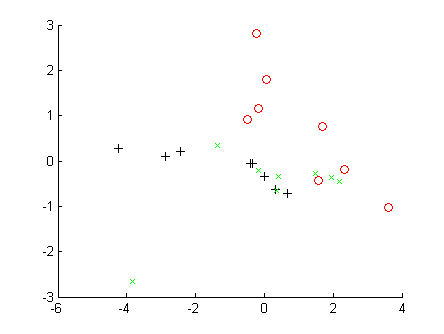
\includegraphics[width=110mm]{paclassplot.png}
\caption{Scatter plot shows dependency between first two principal components used and actual class of an object. Black plus signs indicate "paper" sign , green crosses indicate "rock" sign, red circles indicate "scissors" sign. }
\label{fig:paclassplot}
\end{center}
\end{figure}

Cross validation test results showed that best accuracy over validation data set was achieved by using combination of Hu moments and temporal area of the extracted object as features of the motion image and multi-class SVM for classification. Results for using different feature sets are shown in Table \ref{tab:features}, for using different number of principal components are shown in Table \ref{tab:pca} and for using different classifiers in Table \ref{tab:classify}.

\begin{table}
\begin{center}
\begin{tabular}{| l | r | r |}
\hline
Features & Test set & Validation set \\ \hline
Temporal area of object only & 73.9\% & 54.2\% \\
Hu moments only & 79.3\% & 58.3\% \\
Both & 91.6\% & 87.5\% \\
\hline
\end{tabular}
\end{center}
\caption{Cross validation results when using different sets of features with optimal number of principal components and optimal classifier.}
\label{tab:features}
\end{table}


\begin{table}
\begin{center}
\begin{tabular}{| l | r | r |}
\hline
Number of PC & Test set & Validation set \\ \hline
3 & & \% \\
4 & & \% \\
5 & & 87.5\% \\
6 & & \% \\
7 & & \% \\
\hline
\end{tabular}
\end{center}
\caption{Cross validation results when using different number of principal components with set of features and optimal classifier.}
\label{tab:pca}
\end{table}

\begin{table}
\begin{center}
\begin{tabular}{| l | r | r |}
\hline
Number of PC & Test set & Validation set \\ \hline
RBF & &  \\
MLP & &  \\
Multi-class SVM & & 87.5\% \\
\hline
\end{tabular}
\end{center}
\caption{Cross validation results when using different classifiers with optimal set of features and optimal number of principal components.}
\label{tab:classify}
\end{table}


\section{Source code}

\lstset{numbers=left, stepnumber=2}
\lstinputlisting[language=python, breaklines=true, title=\textbf{'Python Script for general hand recognition  and feature extraction'}]{./../Program.py}
\newpage
\lstset{numbers=left, stepnumber=2}
\lstinputlisting[language=python, breaklines=true, title=\textbf{'Python Script for Classification, training and evaluation'}]{./../classify.py}
\newpage
\lstset{numbers=left, stepnumber=2}
\lstinputlisting[language=python, breaklines=true, title=\textbf{'Python Script for general utility functions'}]{./../av_utils.py}
\newpage
\lstset{numbers=left, stepnumber=2}
\lstinputlisting[language=python, breaklines=true, title=\textbf{'Python Script for Motion History Image construction based on OpenCV sample'}]{./../mhi_update.py}

\end{document}
